\documentclass{article}
\usepackage{ws_template}
\usepackage{amsmath}
\usepackage{amssymb}
\usepackage{graphicx}


\title{homework sheet 08}


\author{
	\name{Denys Sobchyshak}\\
	\imat{03636581}\\
	\email{denys.sobchyshak@tum.de}
	\And
	\name{Sergey Zakharov} \\
	\imat{03636642}\\
	\email{ga39pad@mytum.de}
}

\begin{document}
\maketitle
\textbf{Problem 1:} \\
Distance to a training sample in the feature space is given by:
$$|\phi(x)-\phi(x^{(s_i)})|_2$$
Since replacing this by squred distance doesn't change which points are nearest to x, we get:
$$|\phi(x)-\phi(x^{(s_i)})|_2^2=(\phi(x)-\phi(x^{(s_i)}))^T(\phi(x)-\phi(x^{(s_i)}))= \phi(x)^T\phi(x)-2\phi(x)^T\phi(x^{(s_i)})+\phi(x^{(s_i)})^T\phi(x^{(s_i)}).$$
Since the first term is a constant we can drop the it and must find the k training samples $x^{(si)}$ that minimizes
$$\phi(x^{(s_i)})^T\phi(x^{(s_i)})-2\phi(x)^T\phi(x^{(s_i)})=K(x^{(s_i)}, x^{(s_i)})-2K(x,x^{(s_i)})$$
\\

\textbf{Problem 2:} \\
Definition of a convex function $f(x)$ is:
\begin{equation}
f( \alpha_1 x_1 + \alpha_2 x_2 )   \le    \alpha_1 f( x_1 ) + \alpha_2 f( x_2 ),
\end{equation}

of a convex function $g(x)$:

\begin{equation}
g( \alpha_1 x_1 + \alpha_2 x_2 )   \le    \alpha_1 g( x_1 ) + \alpha_2 g( x_2 ).
\end{equation}

\begin{equation}
h( x )   =    f(x) + g(x),
\end{equation}

so

\begin{equation}
h( \alpha_1 x_1 + \alpha_2 x_2 ) = f( \alpha_1 x_1 + \alpha_2 x_2 ) + g( \alpha_1 x_1 + \alpha_2 x_2 ),
\end{equation}

for which from (1) and (2) the following inequality holds:

\begin{equation}
f( \alpha_1 x_1 + \alpha_2 x_2 ) + g( \alpha_1 x_1 + \alpha_2 x_2 )   \le    \alpha_1 f( x_1 ) + \alpha_2 f( x_2 ) + \alpha_1 g( x_1 ) + \alpha_2 g( x_2 ),
\end{equation}

where the rhs:

\begin{equation}
\alpha_1 f( x_1 ) + \alpha_2 f( x_2 ) + \alpha_1 g( x_1 ) + \alpha_2 g( x_2 ) = \alpha_1 h( x_1 ) + \alpha_2 h( x_2 ).
\end{equation}

We get:

\begin{equation}
h( \alpha_1 x_1 + \alpha_2 x_2 ) \le \alpha_1 h( x_1 ) + \alpha_2 h( x_2 ),
\end{equation}

which is exactly the definition of a convex function.\\
Let's consider function $u(x)=cf(x)$ with $c\ge0$

\begin{equation}
f( \alpha_1 x_1 + \alpha_2 x_2 )   \le    \alpha_1 f( x_1 ) + \alpha_2 f( x_2 ),
\end{equation}

consequently:

\begin{equation}
cf( \alpha_1 x_1 + \alpha_2 x_2 )   \le    c\alpha_1 f( x_1 ) + c\alpha_2 f( x_2 ),
\end{equation}

which is:

\begin{equation}
u( \alpha_1 x_1 + \alpha_2 x_2 )   \le    \alpha_1 u( x_1 ) + \alpha_2 u( x_2 ),
\end{equation}
\\

\setcounter{equation}{0}
\textbf{Problem 3:} \\
Let's take two functions $f_1(x)$ and $f_1(x)$ from the family of covex functions and prove that $g_1(x) = \max(f_1(x) + f_2(x))$ is convex. If this holds, then the pointwise maximum of whole family is convex.

\begin{align} \nonumber
g_1( \alpha_1 x_1 + \alpha_2 x_2 )  &= \max(f_1( \alpha_1 x_1 + \alpha_2 x_2 ), f_2( \alpha_1 x_1 + \alpha_2 x_2 ))\\ \nonumber
&\le \max(\alpha_1 f_1( x_1 ) + \alpha_2 f_1( x_2 ), \alpha_1 f_2( x_1 ) + \alpha_2 f_2( x_2 ))\\ \nonumber
&\le \max(\alpha_1 f_1( x_1 ), \alpha_1 f_2( x_1 )) + \max(\alpha_2 f_1( x_2 ) + \alpha_2 f_2( x_2 ))\\ \nonumber
&= \alpha_1 g_1(x_1) + \alpha_2 g_1(x_2)
\end{align}
\\

\textbf{Problem 4:} \\
The Lagrangian is given by
$$L(x,\alpha) = f_0(x)+\sum_{i}\alpha_if_i(x).$$
Which can be interpreted as a family of functions $L_x(\alpha)=L(x,\alpha)$, that means we interpret $x$ as fixed. Thus $L_x(\alpha)$ has the form:
$$L_x(\alpha)=C_{0,x}+\sum_{i}C_{i,x}\alpha_i$$
where $C_s$ are constants. By applying the definition of a convex function that
$L_x(\alpha)$ is convex for any $C_s$.

The Lagrange dual function is given by the pointwise minimum of this family of functions,
$$g(\alpha) = \min_x L(x,\alpha) = \min_x L_x(\alpha) = − \max_x(−L_x(\alpha)).$$
The negative Lagragian $−L_x(\alpha)$ is also convex because the negation only changes the sign of constants $C_{0,x}$ and $C_{i,x}$. Thus $−g(\alpha)$ is convex and $g(\alpha)$ is concave.
\\

\textbf{Problem 5:} \\
\begin{center}
	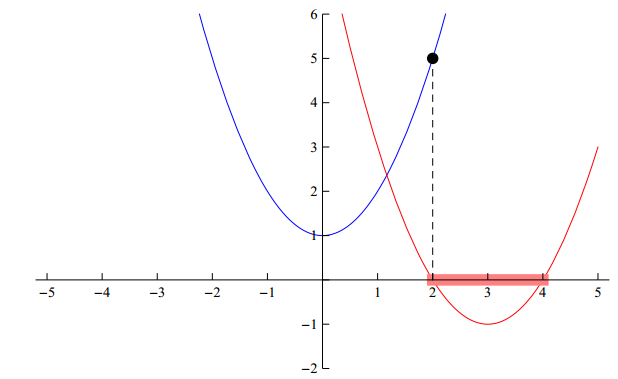
\includegraphics[scale=0.3]{img1}
\end{center}
The objective $f_0(x)$ is in blue, the constraint $f_1(x)$ in red. The feasible region $[2, 4]$ is marked in pink. As $f_0(x)$ is increasing with $|x|$ the minimizer $x_{\star}$ is at the smallest $|x|$ that is in the feasible region. Thus $x_{\star} = 2$ minimizes the optimization problem with the minimal value $f_0(2) = 5$.
\\

\textbf{Problem 6:}\\
The Lagrangian is given by
$$L(x,\alpha) = f_0(x) + \alpha f_1(x) = x^2+1+\alpha(x-2)(x-4)$$
\begin{center}
	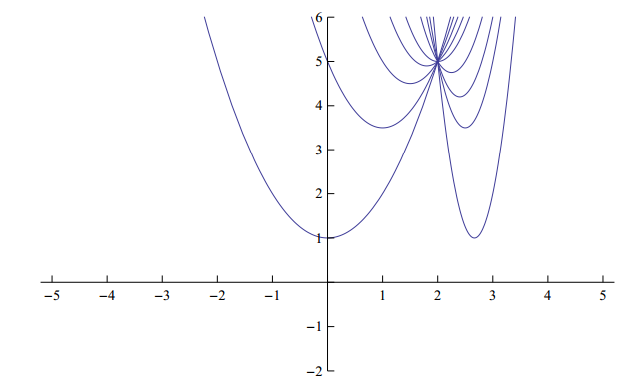
\includegraphics[scale=0.3]{img2}
\end{center}

The plot series shows raising $\alpha$ from left to right.

The Lagrangian is larger for all regions where the constraint is violated, because then $f_1(x)>0$ and $\alpha$ is positive, and smaller for all regions where the constraint is satisfied. Points for which constraint is satisfied with equality, $f_1(x) = 0$, are unaffected. Thus it penalizes the target function at regions where the constraint is violated to amount controlled by the Lagrange multiplier $\alpha$.
\\

\textbf{Problem 7:}\\
We calculate the minimum of $L(x, \alpha)$ w.r.t. $x$,
$$\frac{\partial L}{\partial x} = 2x+\alpha[(x-4)+(x-2)] = (2+2\alpha)x-6\alpha = 0$$
$$\Rightarrow x_{min}(\alpha) = \frac{3\alpha}{\alpha+1}.$$
The Lagrange dual function is given by
$$g(\alpha) = L(x_{min}(\alpha), \alpha) = 10-\alpha-\frac{9}{1+\alpha}$$

\begin{center}
	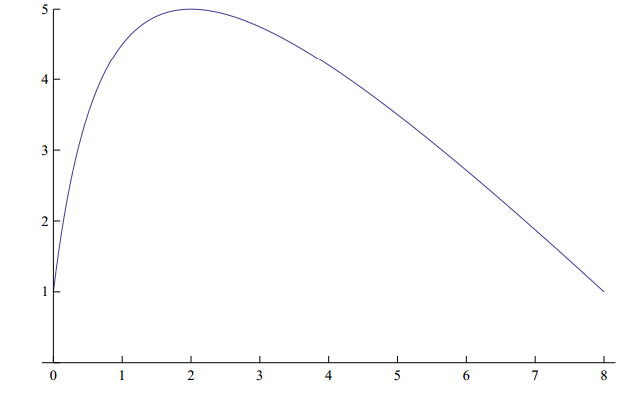
\includegraphics[scale=0.3]{img3}
\end{center}

The dual problem is
$$\text{maximize }g(\alpha) = 10-\alpha-\frac{9}{1+\alpha}$$
$$\text{subject to }\alpha \geq 0$$
\\

\textbf{Problem 8:}\\
The dual function $g(\alpha)$ is concave, thus its maximums are given by
$$\frac{dg}{d\alpha}=-1+9(1+\alpha)^{-2}=0$$
$$(1+\alpha)^2 = 9$$
$$1+\alpha = \pm3$$
$$\Rightarrow \alpha_1 = 2$$
$$\Rightarrow \alpha_2 = -4$$
Only $\alpha_1$ satisfies the constraint $\alpha\geq 0$, thus the dual optimal solution is $\alpha^{\star} = 2$ and the dual optimal value is $g(\alpha^{\star}) = 5$.
\\

\textbf{Problem 9:}\\
Yes, it is. $f_0$ and $f_1$ are both convex and at the point $x = 3$ we have $f_1(3) < 0$. Thus Slater's constraint qualification applies and the duality gap is zero.
\\

\textbf{Problem 10:}\\
Constraint $f_1$ is active because the corresponding Lagrange multiplier $\alpha^{\star} = 2$ is not zero.

If a constraint is active thus it limits the solution, that is if the constraint was dropped we could obtain a lower value of the objective function.


\end{document}
